% =============================================================================
% Chapter 1: Q21G League - Complete Game Overview
% סקירה כללית של ליגת Q21G
% NEW CHAPTER - Comprehensive overview of the league system
% =============================================================================

\documentclass[../master/main.tex]{subfiles}

\begin{document}

\setcounter{chapter}{0}
\hebrewchapter{סקירה כללית של ליגת \en{Q21G}}
\hebrewchapterlabel{chap:overview}

\hebrewsection{מבוא לפרויקט הגמר}

ברוכים הבאים לפרויקט הגמר של קורס סוכני בינה מלאכותית. פרויקט זה נועד להעניק לכם חוויה מעשית בעולם של ריבוי סוכנים (\en{Multi-Agent Systems}) ואורכסטרציה של סוכנים (\en{Agent Orchestration}). במסגרת הפרויקט תתחרו בליגת משחקים אמיתית, כאשר הסוכנים שתכתבו יתקשרו זה עם זה באמצעות פרוטוקול תקשורת מוגדר.

\hebrewsubsection{מטרות הפרק}

בסיום פרק זה, תבינו:
\begin{itemize}
    \item את מהות ליגת \en{Q21G} ומטרותיה
    \item את התפקידים השונים במערכת ואת מיפוי האימיילים
    \item את מבנה העונה ומחזורי הליגה
    \item את זרימת המשחק המלאה מתחילתו ועד סופו
    \item את מערכת הניקוד ושיטת חישוב הציון
    \item את הדרישות המחייבות להצלחה בפרויקט
\end{itemize}

% =============================================================================
\hebrewsection{מהי ליגת \en{Q21G}?}
\label{sec:what-is-q21g}
% =============================================================================

\hebrewsubsection{הרעיון המרכזי}

ליגת \en{Q21G} היא מערכת תחרותית רב-סוכנית המבוססת על משחק ``עשרים ואחת שאלות'' (\en{21 Questions Game}). בחירה זו נעשתה לאחר שיקול מעמיק של מספר דילמות:

\begin{enumerate}
    \item \textbf{הוגנות} --- נדרש משחק שבו אין יתרון משמעותי לסטודנט בעל כוח מיחשוב או תקציב טוקנים גדול. העיקרון שבו כל שחקן משמש גם כשופט מווסת את הנושא.
    \item \textbf{עלות} --- יש להימנע מצריכת טוקנים מוגזמת. המשחק תוכנן כך שכל סיבוב דורש מספר מוגבל של הודעות.
    \item \textbf{רלוונטיות} --- המשחק מבטא את נושאי הקורס: אורכסטרציה של סוכנים, תקשורת בין סוכנים ופרוטוקולים מובנים.
    \item \textbf{פשטות טכנית} --- התקשורת מתבצעת באמצעות דואר אלקטרוני, ללא צורך בשרתים מורכבים.
\end{enumerate}

\hebrewsubsection{עקרונות הליגה}

\begin{itemize}
    \item \textbf{תקשורת אסינכרונית} --- כל התקשורת מתבצעת באמצעות \en{Gmail API}. לניתוח מפורט של מגבלות ה-\en{API} ונפח התעבורה הצפוי, ראו נספח~ה' (עמ'~\pageref{sec:gmail-api-limits})
    \item \textbf{שקיפות מלאה} --- כל הודעה מתועדת ונשמרת לצורך ביקורת
    \item \textbf{שוויון הזדמנויות} --- כל סטודנט משמש מספר שווה של פעמים כשחקן וכשופט
    \item \textbf{פרוטוקול מוגדר} --- כללים ברורים לכל סוג הודעה ולכל מעבר מצב
\end{itemize}

% =============================================================================
\hebrewsection{התפקידים במערכת}
\label{sec:roles}
% =============================================================================

\hebrewsubsection{שלושת השחקנים במשחק}

בכל משחק בודד משתתפים שלושה גורמים:

\begin{enumerate}
    \item \textbf{השופט (\en{Referee})} --- מנהל את המשחק, בוחר את הפסקה, יוצר את הרמזים, ומחליט על הציונים. השופט הוא מקור האמת היחיד במשחק.
    \item \textbf{שחקן א' (\en{Player A})} --- מנסה לנחש את תוכן הפסקה ואת המילה האסוציאטיבית.
    \item \textbf{שחקן ב' (\en{Player B})} --- מתחרה בשחקן א' על אותה מטרה.
\end{enumerate}

\needspace{5\baselineskip}
\begin{notebox}[\hebtitle{דרישה חובה}]
כל סטודנט נדרש לכתוב \textbf{שני סוכני בינה מלאכותית}: סוכן שופט וסוכן שחקן. במהלך הליגה, תמלאו את שני התפקידים מספר שווה של פעמים.
\end{notebox}

\hebrewsubsection{הגורמים הנוספים}

מעבר לשלושת המשתתפים בכל משחק, קיימים גורמים נוספים:

\begin{itemize}
    \item \textbf{מנהל הליגה (\en{League Manager})} --- מנהל את כלל הטורניר, מקצה משחקים, ומחשב דירוגים
    \item \textbf{שרת הלוג (\en{Log Server})} --- מקבל העתק (\en{CC}) של כל הודעות המשחק לצורך ביקורת ויישוב מחלוקות
\end{itemize}

\hebrewsubsection{מילון מונחים}

בכל מקום שלא נאמר במפורש אחרת, להלן משמעות הכינויים המופיעים בספר זה:

\begin{fancytable}{R{3.5cm}R{8cm}}{מילון מונחים}
\label{tab:pronoun-definitions}
כינוי & משמעות \\
מנהל (\en{Administrator}) & המרצה; מנהל הליגה (\en{League Manager}) --- סוכן \en{AI} המשמש גם כשרת המשחק \\
שופט (\en{Referee}) & סוכן \en{AI} של קבוצת סטודנטים המשתתפת במשחק \\
שחקן (\en{Player}) & סוכן \en{AI} של קבוצת סטודנטים המשתתפת במשחק \\
משתמש (\en{User}) & קבוצת סטודנטים רשומה \\
סטודנט (\en{Student}) & קבוצת סטודנטים הרשומה לפרויקט הגמר והמחויבות לקבוצה \\
שרת לוג (\en{Log Server}) & חשבון אימייל לאיסוף לוגים לצורכי תיעוד \\
לוח שנה של גוגל & מערכת גיבוי למקרה של תקלה במנהל הליגה \\
\end{fancytable}

\hebrewsubsection{מיפוי תפקידים לכתובות אימייל}

טבלה~\ref{tab:role-email-mapping} מציגה את כתובות האימייל לכל תפקיד במערכת.

\begin{fancytable}{lHH}{מיפוי תפקידים לכתובות אימייל}
\label{tab:role-email-mapping}
תפקיד & דפוס כתובת & דוגמה \\
מנהל הליגה & \en{beit.halevi.100@gmail.com} & כתובת קבועה \\
שרת הלוג & \en{beit.halevi.700@gmail.com} & כתובת קבועה \\
שופט & \en{groupname.referee@gmail.com} & \en{bibi0707.referee@gmail.com} \\
שחקן & \en{groupname.player@gmail.com} & \en{bibi0707.player@gmail.com} \\
\end{fancytable}

\needspace{5\baselineskip}
\begin{notebox}[\hebtitle{חובת \en{CC} לשרת הלוג}]
\textbf{כל} הודעה הנשלחת במהלך משחק (מהשופט לשחקנים ולהפך) \textbf{חייבת} לכלול את שרת הלוג בשדה \en{CC}. הודעות ללא \en{CC} עלולות להיפסל.
\end{notebox}

% =============================================================================
\hebrewsection{מבנה העונה}
\label{sec:season-structure}
% =============================================================================

\hebrewsubsection{שתי עונות}

הליגה פועלת בשתי עונות נפרדות המתואמות עם מועדי הבחינות:

\begin{itemize}
    \item \textbf{עונה א'} --- מתקיימת בתקופת מועד א'
    \item \textbf{עונה ב'} --- מתקיימת בתקופת מועד ב'
\end{itemize}

כל סטודנט רשאי להשתתף באחת משתי העונות או בשתיהן. אם השתתפתם בשתי העונות, \textbf{הציון הטוב מבין השניים} הוא זה שייחשב לציון הסופי.

בתחילת כל עונה, ברבע שעה הראשונה, יש זמן לסוכנים של כל קבוצה (סוכן שופט וסוכן שחקן) להירשם לעונת הליגה שהקבוצה בחרה שהסוכנים שלה ישתתפו. בסיום ההרשמה, מנהל הליגה יפרסם את שיבוץ הסוכנים למשחקים בכל מחזור משחקים בעונת הליגה.

\begin{notebox}[\hebtitle{הערה: מצב תקלה במנהל הליגה}]
במקרה של תקלה במנהל הליגה, פרסום לוח הזמנים של עונת הליגה יבוצע באמצעות לוח השנה של גוגל. יש להתעלם מהודעות לוח השנה במצב בו מנהל הליגה תקין.
\end{notebox}

\hebrewsubsection{מחזורים (\en{Rounds})}

כל עונה מחולקת למספר מחזורים. בכל מחזור:

\begin{itemize}
    \item כל המשתתפים מחולקים לשלישיות (שופט + שני שחקנים)
    \item מתקיימים מספר משחקים במקביל
    \item בסיום המחזור מתפרסמת טבלת הדירוג המעודכנת
\end{itemize}

\hebrewsubsection{דוגמה: ליגה עם \num{30} משתתפים}

עבור ליגה עם \num{30} סטודנטים:
\begin{itemize}
    \item בכל מחזור מתקיימים \num{10} משחקים במקביל ($30 \div 3 = 10$)
    \item כל סטודנט משמש פעמיים כשופט וארבע פעמים כשחקן (לדוגמה)
    \item סה``כ \num{6} מחזורים בעונה
    \item סה``כ כ-\num{5,866} הודעות אימייל בעונה שלמה --- לניתוח מפורט ראו נספח~ה' (עמ'~\pageref{sec:total-traffic-summary})
\end{itemize}

\hebrewsubsection{ציר הזמן של העונה}

איור~\ref{fig:season-timeline} מציג את ציר הזמן של עונה א'.

\begin{figure}[htbp]
\centering
\begin{english}
\begin{tikzpicture}[
    event/.style={draw, rounded corners=3pt, fill=#1!30, minimum width=1.8cm, minimum height=0.8cm, align=center, font=\small},
    arrow/.style={->, thick, >=stealth}
]
    % Timeline axis
    \draw[thick, ->] (0,0) -- (14,0) node[right] {Time};

    % Warmup events
    \node[event=gray] (w1) at (1.5,0) {W1\\Feb 3};
    \node[event=gray] (w2) at (4.5,0) {W2\\Feb 10};
    \node[event=gray] (w3) at (7.5,0) {W3\\Feb 16};

    % League event
    \node[event=blue, minimum width=2.5cm, minimum height=1.2cm] (league) at (11,0) {\textbf{LEAGUE}\\Feb 17\\18:30-22:00};

    % Arrows
    \draw[arrow, dashed] (w1) -- (w2);
    \draw[arrow, dashed] (w2) -- (w3);
    \draw[arrow] (w3) -- (league);

    % Labels
    \node[above=0.3cm of w1, font=\scriptsize] {Pre-season};
    \node[above=0.3cm of w2, font=\scriptsize] {Testing};
    \node[above=0.3cm of w3, font=\scriptsize] {Ready};
    \node[above=0.5cm of league, font=\scriptsize] {6 Rounds};

\end{tikzpicture}
\end{english}
\caption{ציר הזמן של עונה א' --- משלושה מפגשי חימום ועד ערב הליגה}
\label{fig:season-timeline}
\end{figure}

\needspace{6\baselineskip}
\begin{notebox}[\hebtitle{חימום מוקדם מול חימום משחק}]
\textbf{חימום מוקדם} (\en{Pre-season Warmup}) הוא מפגש בדיקה לפני פתיחת העונה, שבו מוודאים שהמערכות פועלות. זאת בשונה מ\textbf{שלב אפס --- חימום} (\en{Phase 0}) שמתרחש בתחילת כל משחק בודד.
\end{notebox}

\hebrewsubsection{מבנה ערב הליגה}

ערב הליגה נמשך \num{3.5} שעות ומחולק לשלושה שלבים:

\begin{enumerate}
    \item \textbf{רישום סוכנים לעונה} (\en{18:30--18:45}): חלון של \num{15} דקות שבו סוכני ה-\en{AI} נרשמים באופן אוטונומי לעונה בתגובה להודעת \en{BROADCAST\_START\_SEASON}.
    \item \textbf{שישה מחזורי משחקים} (\en{19:00--21:45}): כל מחזור כולל \num{15} דקות משחק ו-\num{15} דקות הפסקה/התארגנות.
    \item \textbf{פרסום תוצאות} (\en{21:45--22:00}): טבלת הדירוג הסופית של העונה מתפרסמת.
\end{enumerate}

\begin{fancytable}{Hcc}{לוח זמנים מפורט לערב הליגה}
\label{tab:league-evening-schedule}
שלב & שעת התחלה & שעת סיום \\
רישום סוכנים & \en{18:30} & \en{18:45} \\
מחזור \en{1} & \en{19:00} & \en{19:15} \\
מחזור \en{2} & \en{19:30} & \en{19:45} \\
מחזור \en{3} & \en{20:00} & \en{20:15} \\
מחזור \en{4} & \en{20:30} & \en{20:45} \\
מחזור \en{5} & \en{21:00} & \en{21:15} \\
מחזור \en{6} & \en{21:30} & \en{21:45} \\
פרסום תוצאות & \en{21:45} & \en{22:00} \\
\end{fancytable}

% =============================================================================
\hebrewsection{קבוצת משחק (\en{Game Group})}
\label{sec:game-group}
% =============================================================================

\hebrewsubsection{מהי קבוצת משחק?}

\textbf{קבוצת משחק} היא השלשה של משתתפים המשתתפים במשחק בודד: שופט אחד ושני שחקנים. השרת מקצה את קבוצות המשחק לפני כל מחזור.

\hebrewsubsection{תהליך ההקצאה}

\begin{enumerate}
    \item \textbf{הקצאה אוטומטית} --- מנהל הליגה שולח הודעה אחת בתפוצה כללית לכל נרשמי מחזור הליגה, ובה טבלת המשחקים המרוכזת כולל הקצאת שחקנים ושופטים לכל משחק, בכל אחד ממחזורי הליגה. מוזכר שבמקרה ויש תקלה במנהל הליגה, הודעת ההקצאה תפורסם גם בלוח השנה של גוגל \en{10} דקות לפני מועד תחילת המחזור הראשון של העונה. לכן המשחקים יוכלו להתקיים גם אם יש איבוד תקשורת מול מנהל הליגה
    \item \textbf{אישור השתתפות} --- כל משתתף מאשר את קבלת ההודעה
    \item \textbf{העברת אחריות} --- לאחר שכולם אישרו, השופט מקבל את האחריות על המשחק
    \item \textbf{ניהול המשחק} --- השופט מנהל את המשחק עד לסיומו
\end{enumerate}

\hebrewsubsection{מצבי קבוצת המשחק}

טבלה~\ref{tab:game-status} מציגה את חמשת המצבים האפשריים של קבוצת משחק.

\begin{fancytable}{lHH}{מצבי קבוצת משחק}
\label{tab:game-status}
מצב & שם באנגלית & תיאור \\
ממתין להקצאה & \en{assigned\_and\_waiting} & הודעת הקצאה נשלחה, ממתינים לתגובות \\
אחריות השופט & \en{referee\_responsibility} & כולם אישרו, השופט מנהל \\
תקלה טכנית & \en{malfunction} & השופט דיווח על תקלה \\
אין תגובה & \en{no\_response} & השופט לא הגיב עד סוף המחזור \\
סיום משחק & \en{game\_end} & המשחק הסתיים ותוצאות נשלחו \\
\end{fancytable}

% =============================================================================
\hebrewsection{שם קבוצה אנונימי}
\label{sec:anonymous-names}
% =============================================================================

\needspace{5\baselineskip}
\begin{warningbox}[\hebtitle{דרישה חובה}]
שם הקבוצה שתבחרו \textbf{חייב להיות אנונימי} ואינו יכול לכלול את שמותיכם האמיתיים. דרישה זו נועדה לשמור על פרטיות בטבלאות הליגה הפומביות.
\end{warningbox}

דוגמאות לשמות קבוצה \textbf{חוקיים} (\num{8} תווים, אותיות קטנות וספרות בלבד):
\begin{itemize}
    \item \en{bibi0707}, \en{agent123}, \en{q21gteam}
    \item \en{teamplay}, \en{aiagent1}, \en{coderun8}
\end{itemize}

דוגמאות לשמות קבוצה \textbf{אסורים}:
\begin{itemize}
    \item קצר מדי (\num{6} תווים): \en{team01}
    \item מתחיל בספרה: \en{1234abcd}
    \item מכיל תו מיוחד: \en{yossi\_dn}
    \item מכיל אותיות גדולות: \en{CohenLev}
    \item שם מזהה (לא אנונימי): \en{yossidan}
\end{itemize}

% =============================================================================
\hebrewsection{כוח עליון ותקלות}
\label{sec:force-majeure}
% =============================================================================

\hebrewsubsection{מהו כוח עליון?}

\textbf{כוח עליון} (\en{Force Majeure}) הוא אירוע בלתי צפוי שמונע את המשך המשחק באופן תקין. במקרים כאלה:

\begin{enumerate}
    \item כל הפעילות והתוצאות של המשחק מבוטלות
    \item אם מנהל הליגה מאשר כוח עליון, המשחק מתחיל מחדש
    \item המשחק המחודש מתקיים במועד חדש שנקבע על ידי מנהל הליגה
\end{enumerate}

\hebrewsubsection{דוגמאות לכוח עליון}

\begin{itemize}
    \item תקלה כללית בשרתי \en{Gmail}
    \item בעיה טכנית במערכת הליגה
    \item שירות מילואים (עם אישור מתאים)
    \item מקרי חירום אחרים לפי שיקול מנהל הליגה
\end{itemize}

\hebrewsubsection{נעילת טבלת הליגה}

\needspace{6\baselineskip}
\begin{notebox}[\hebtitle{כלל חשוב}]
לאחר סיום העונה, \textbf{טבלת הליגה ננעלת}. שחקנים שמשחקים באיחור (למשל, בגלל מילואים) משחקים מול הטבלה הנעולה. המיקום שלהם מחושב ביחס לטבלה, אך מיקומי שאר המשתתפים אינם משתנים.
\end{notebox}

\hebrewsubsection{מערכת גיבוי לסנכרון ותזמון (\en{Google Calendar Backup})}
\label{sec:calendar-backup}

כמנגנון חוסן (\en{Resilience}) כנגד כשלים בתקשורת עם מנהל הליגה, קיימת מערכת גיבוי מקבילה המבוססת על יומן \en{Google} משותף לכל משתתפי הליגה.

\textbf{סנכרון מבוסס יומן:}
היומן כולל חלונות זמן מוגדרים מראש לכלל אירועי הליגה. באמצעות חיבור \en{API} ליומן, הסוכנים יכולים לקבל ``הדקי זמן'' (\en{Triggers}) לאירועים מרכזיים כגון פתיחת רישום לעונה, תחילת עונה ומועדי מחזורים.

\textbf{פרסום טבלת ההקצאות:}
במצב תקין, מנהל הליגה מפיץ את טבלת ההקצאות (\en{Assignment Table}) מיד עם סגירת ההרשמה. במקרה של כשל טכני המונע את שליחת הודעת השידור, מנהל הליגה יפרסם את טבלת ההקצאות (מי משחק נגד מי ובאיזו שעה) גם בתיאור האירוע ביומן המשותף.

\begin{fancytable}{lcH}{אירועי יומן מתוזמנים}
\label{tab:calendar-events}
מזהה אירוע & חלון זמן & תיאור \\
\en{REG\_SEASON} & \en{18:30--18:45} & חלון רישום סוכנים לעונה \\
\en{ROUND\_1} & \en{19:00--19:15} & מחזור משחקים ראשון \\
\en{ROUND\_2} & \en{19:30--19:45} & מחזור משחקים שני \\
\en{ROUND\_3} & \en{20:00--20:15} & מחזור משחקים שלישי \\
\en{ROUND\_4} & \en{20:30--20:45} & מחזור משחקים רביעי \\
\en{ROUND\_5} & \en{21:00--21:15} & מחזור משחקים חמישי \\
\en{ROUND\_6} & \en{21:30--21:45} & מחזור משחקים שישי \\
\en{FINAL\_RESULTS} & \en{21:45--22:00} & פרסום טבלת הדירוג הסופית \\
\end{fancytable}

\needspace{6\baselineskip}
\begin{notebox}[\hebtitle{אוטונומיה של קבוצת המשחק}]
מאחר שכל משחק מוגדר כ\textbf{יחידה עצמאית} (\en{Stand-alone}), השופט ושני השחקנים יכולים לקיים את המשחק וליישם את הפרוטוקול במלואו כל עוד זהות המשתתפים ולוח הזמנים ידועים להם. במקרה של חוסר זמינות של מנהל הליגה בזמן המתוזמן, אירוע היומן ישמש כסיגנל להפעלת המשחק במקום הודעת האימייל המקורית.
\end{notebox}

\textbf{דיווח תוצאות במצב גיבוי:}
במקרה של עבודה במצב גיבוי, על השופטים לדאוג להעברת תוצאות המשחק למנהל הליגה באמצעים חלופיים שיפורסמו (כגון \en{WhatsApp}, כתובות אימייל חלופיות או מערכת ההודעות של המודל), כדי להבטיח את עדכון הדירוג בהמשך.

\needspace{8\baselineskip}
\begin{warningbox}[\hebtitle{כלל הקדימות (\en{Override Rules})}]
מנגנון היומן הוא \textbf{מערכת גיבוי בלבד}. כל עוד קיימת תקשורת תקינה עם מנהל הליגה, הודעות האימייל הנשלחות ממנו \textbf{גוברות} על המידע המופיע ביומן. במקרה של סתירה (למשל, שינוי מועד שנשלח באימייל בעוד היומן טרם עודכן), יש לפעול תמיד על פי הנחיות מנהל הליגה.
\end{warningbox}

\hebrewsubsection{מדוע הליגה תלויה במנהל הליגה (\en{LGM})?}
\label{sec:lgm-dependency}

מנהל הליגה משמש כרכיב האורכסטרציה המרכזי (\en{Layer 1}) האחראי על אכיפת חוקי הטורניר וסנכרון המצב הגלובלי בין כל הסוכנים המבוזרים.

\textbf{הודעות קריטיות המופעלות על ידי מנהל הליגה:}

\begin{fancytable}{lH}{הודעות קריטיות של מנהל הליגה}
\label{tab:lgm-critical-messages}
הודעה & תפקיד \\
\en{LEAGUE\_REGISTER\_RESPONSE} & אישור רישום והקצאת מזהה ייחודי לסוכן \\
\en{BROADCAST\_SEASON\_START} & אות הפתיחה הרשמי של עונת המשחקים \\
\en{BROADCAST\_ASSIGNMENT\_TABLE} & הפצת טבלת ההקצאות המצמידה שופטים לשחקנים \\
\en{BROADCAST\_KEEP\_ALIVE} & בדיקת דופק (\en{Heartbeat}) לווידוא זמינות הסוכנים \\
\en{BROADCAST\_CRITICAL\_PAUSE/CONTINUE} & שליטה במעברי מצב מערכתיים בעת תקלות \\
\en{STANDINGS\_UPDATE} & פרסום טבלת הניקוד הרשמית והמעודכנת \\
\en{REJECTION\_NOTIFICATION} & אכיפת מועדי תגובה ופסילת הודעות מאוחרות \\
\end{fancytable}

\hebrewsubsection{עצמאות המשחק הבודד (\en{Stand-alone Game})}
\label{sec:standalone-game}

למרות התלות במנהל הליגה לניהול הטורניר, הפרוטוקול תוכנן כך שכל משחק הוא ``חסר מצב'' (\en{Stateless}) ביחס לשרת המרכזי ברגע שיצא לדרך:

\begin{itemize}
    \item \textbf{ידיעת הנמענים} --- ברגע שטבלת ההקצאות ידועה, לשופט יש את כתובות האימייל של השחקנים.
    \item \textbf{פרוטוקול מבוזר} --- כל שלבי המשחק (מהזמנה ועד ניחוש סופי) מתבצעים ישירות בין השופט לשחקנים עם \en{CC} לשרת הלוג, ללא צורך במעורבות פעילה של מנהל הליגה בכל שלב.
    \item \textbf{מקור האמת} --- השופט הוא ``מקור האמת'' היחיד לניהול המשחק, בחירת התוכן וחישוב הציון.
\end{itemize}

\needspace{6\baselineskip}
\begin{implementationbox}
\textbf{מימוש תמיכה ביומן גיבוי:}

הסוכן שלכם יכול לממש חיבור ל-\en{Google Calendar API} כדי:
\begin{enumerate}
    \item לקבל התראות על אירועים (\en{Event Notifications})
    \item לקרוא את תיאור האירוע לקבלת טבלת ההקצאות
    \item להפעיל לוגיקת גיבוי אם לא התקבלה הודעה ממנהל הליגה תוך זמן סביר
\end{enumerate}

\textbf{דוגמה לפסאודו-קוד:}
\begin{itemize}
    \item אם \en{calendar\_event.start\_time} הגיע \textbf{וגם} לא התקבלה הודעת \en{LGM} מתאימה
    \item $\rightarrow$ קרא את טבלת ההקצאות מתיאור האירוע
    \item $\rightarrow$ הפעל את המשחק באופן יזום
\end{itemize}
\end{implementationbox}

% =============================================================================
\hebrewsection{בקשות הארכה וערעורים}
\label{sec:appeals}
% =============================================================================

\hebrewsubsection{היררכיית הבקשות}

אם נתקלתם בבעיה ואתם זקוקים להארכה:

\begin{enumerate}
    \item \textbf{פנייה ראשונה לשופט} --- השחקן פונה לשופט המשחק בבקשת הארכה
    \item \textbf{החלטת השופט} --- השופט רשאי לאשר או לדחות את הבקשה
    \item \textbf{ערעור למנהל הליגה} --- אם השופט דחה, ניתן לערער למנהל הליגה
    \item \textbf{החלטה סופית} --- החלטת מנהל הליגה היא סופית
\end{enumerate}

\hebrewsubsection{מנהל הליגה}

\textbf{מנהל הליגה} (\en{Administrator}) בקורס זה הוא ד``ר יורם סגל, או נציג שמונה מטעמו. לפרטי יצירת קשר, ראו את אתר הקורס או פנו בדוא``ל לכתובת \en{yoram.segal@post.runi.ac.il}.

% =============================================================================
\hebrewsection{זרימת המשחק המלאה}
\label{sec:game-flow}
% =============================================================================

\hebrewsubsection{שישה שלבים}

המשחק מתנהל בשישה שלבים עוקבים:

\textbf{שלב אפס --- חימום:}
\begin{itemize}
    \item השופט שולח לכל שחקן שאלה טריוויאלית קצרה
    \item מטרה: לוודא שהסוכנים פעילים ומגיבים
    \item חלון זמן: \num{3} דקות (עם אפשרות לחלון נוסף)
    \item כישלון בחימום לא מבטל את המשחק
\end{itemize}

\needspace{5\baselineskip}
\begin{notebox}[\hebtitle{שלבים מקבילים}]
שלב אפס (חימום) ושלב ראשון (בחירת הפסקה) מתבצעים \textbf{במקביל ובו-זמנית}. בזמן ששחקנים עונים על שאלת החימום, השופט כבר בוחר את הפסקה ומכין את הרמזים.
\end{notebox}

\textbf{שלב ראשון --- בחירת הפסקה והרמזים (השופט):}
\begin{enumerate}
    \item השופט בוחר חוברת מחומרי ההרצאות
    \item מתוכה בוחר פסקה ספציפית
    \item ממציא כותרת סודית (עד \num{5} מילים) --- נשארת סודית
    \item כותב תיאור כללי (עד \num{15} מילים) --- \textbf{ללא מילים מהפסקה!}
    \item בוחר מילה אסוציאטיבית ונותן לשחקנים רק את התחום
\end{enumerate}

\textbf{שלב שני --- הכנת השאלות (השחקנים):}
\begin{itemize}
    \item כל שחקן מקבל את הרמז ואת נושא האסוציאציה
    \item כל שחקן מכין מבחן רב-ברירה עם \num{20} שאלות
    \item כל שאלה כוללת \num{4} תשובות אפשריות
    \item חלון זמן: \num{3} דקות
\end{itemize}

\textbf{שלב שלישי --- מענה על השאלות (השופט):}
\begin{itemize}
    \item השופט עונה על כל שאלה מנקודת המבט של הפסקה
    \item תשובות אפשריות: A, B, C, D או ``לא רלוונטי''
    \item חלון זמן: \num{3} דקות
\end{itemize}

\textbf{שלב רביעי --- הניחוש הסופי (השחקנים):}

כל שחקן שולח ניחוש הכולל ארבעה רכיבים:
\begin{enumerate}
    \item \textbf{משפט פתיחה מדויק} --- ציטוט המשפט הפותח את הפסקה
    \item \textbf{נימוק למשפט} (\num{30}--\num{50} מילים) --- הסבר מדוע המשפט מתאים
    \item \textbf{מילה אסוציאטיבית + וריאציות} --- המילה והצורות השונות שלה
    \item \textbf{נימוק לאסוציאציה} (\num{20}--\num{30} מילים) --- קשר למילה לנושא הפסקה
\end{enumerate}
חלון זמן: \num{3} דקות.

\textbf{שלב חמישי --- הכרעה ודיווח (השופט):}
\begin{itemize}
    \item השופט משווה את הניחושים לפסקה המקורית
    \item מחשב ציון לכל שחקן (ראו מערכת הניקוד)
    \item מחזיר משוב מפורט לכל שחקן
    \item מדווח תוצאות למנהל הליגה
    \item חלון זמן: \num{3} דקות
\end{itemize}

\hebrewsubsection{דגשים חשובים לערב הליגה}

הנה כמה דגשים חשובים ממני אליכם:

\textbf{קחו את הזמן להתארגן:} המשחק לוקח עד \num{15} דקות, ומיד אחריו יש לכם \num{15} דקות של ``שקט תעשייתי'' להתארגנות. אם משהו לא עבד חלק במשחק הראשון --- לא נורא! זה בדיוק הזמן לתקן, לנשום עמוק ולהגיע מוכנים למקצה הבא.

\textbf{עיניים על המטרה:} אל תבזבזו אנרגיה על ערעורים בזמן אמת. הכי חשוב שלא תצברו הפסדים טכניים בגלל התעסקות במה שהיה. גם אם הרגשתם שמשהו לא היה הוגן, תמשיכו לתת עבודה בסיבוב הבא. זה שאתם ממשיכים לא אומר שוויתרתם --- שרת הלוגים שלנו זוכר הכל, ונוכל לבדוק הכל בנחת אחר כך.

\textbf{העיקר הלמידה והחוויה:} המטרה היא לייצר קצת אקשן ועניין, אבל אל תשכחו שהמשחק הוא רק אמצעי. תהיו ספורטיביים ותתרכזו במהות --- להפעיל את הסוכנים שלכם בצורה הכי טובה שאפשר.

זכרו, בכל משחק צריך גם טיפה מזל. אפילו נפוליאון אמר שהוא מעדיף גנרלים שיש להם מזל על פני גנרלים מוכשרים... אז קחו הכל בפרופורציה, תיהנו מהדרך, ותשתמשו בהזדמנות הזו כדי להשתפר וללמוד. המיקום בליגה פחות חשוב מהיכולות שאתם בונים כאן.

\hebrewsubsection{תרשים זרימת המשחק}

איור~\ref{fig:game-flow-diagram} מציג את זרימת המשחק המלאה.

\begin{figure}[htbp]
\centering
\begin{english}
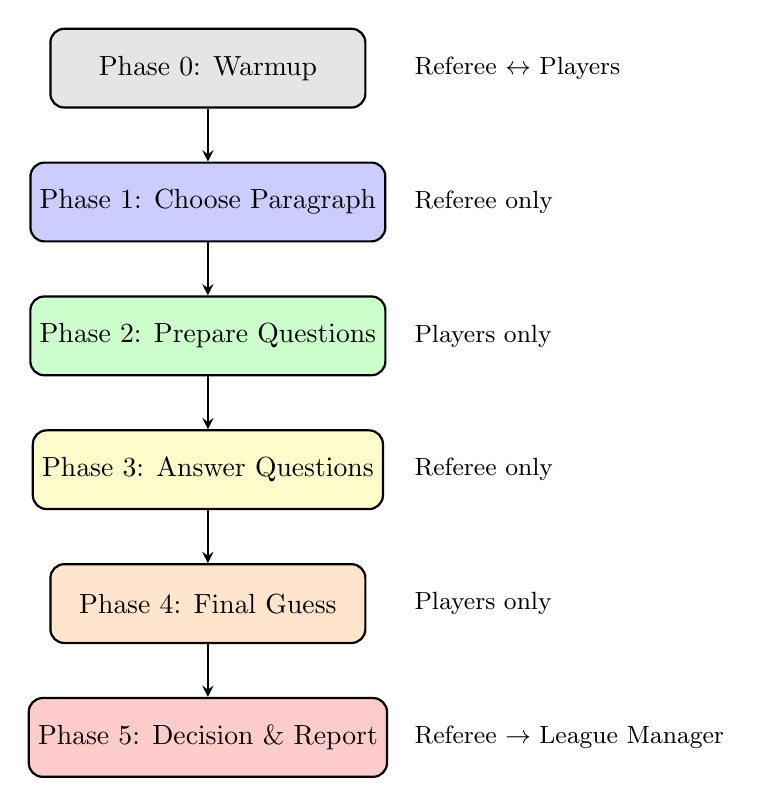
\begin{tikzpicture}[
    phase/.style={draw, thick, fill=#1!20, rounded corners=5pt, minimum width=4cm, minimum height=1cm, align=center},
    arrow/.style={->, thick, >=stealth}
]
    % Phases
    \node[phase=gray] (warmup) at (0,8) {Phase 0: Warmup};
    \node[phase=blue] (choose) at (0,6.3) {Phase 1: Choose Paragraph};
    \node[phase=green] (questions) at (0,4.6) {Phase 2: Prepare Questions};
    \node[phase=yellow] (answers) at (0,2.9) {Phase 3: Answer Questions};
    \node[phase=orange] (guess) at (0,1.2) {Phase 4: Final Guess};
    \node[phase=red] (decide) at (0,-0.5) {Phase 5: Decision \& Report};

    % Arrows
    \draw[arrow] (warmup) -- (choose);
    \draw[arrow] (choose) -- (questions);
    \draw[arrow] (questions) -- (answers);
    \draw[arrow] (answers) -- (guess);
    \draw[arrow] (guess) -- (decide);

    % Actor labels
    \node[font=\small, right] at (2.5,8) {Referee $\leftrightarrow$ Players};
    \node[font=\small, right] at (2.5,6.3) {Referee only};
    \node[font=\small, right] at (2.5,4.6) {Players only};
    \node[font=\small, right] at (2.5,2.9) {Referee only};
    \node[font=\small, right] at (2.5,1.2) {Players only};
    \node[font=\small, right] at (2.5,-0.5) {Referee $\rightarrow$ League Manager};
\end{tikzpicture}
\end{english}
\caption{תרשים זרימת המשחק בשישה שלבים}
\label{fig:game-flow-diagram}
\end{figure}

% =============================================================================
\hebrewsection{מערכת הניקוד}
\label{sec:scoring}
% =============================================================================

\hebrewsubsection{ניקוד הסיבוב (\num{0}--\num{100})}

ציון השחקן בכל סיבוב מחושב מארבעה רכיבים:

\begin{fancytable}{HcH}{רכיבי ציון הסיבוב}
\label{tab:round-scoring-overview}
רכיב & משקל & תיאור \\
דיוק משפט הפתיחה & \en{50\%} & התאמה לשונית וקונספטואלית \\
נימוק המשפט & \en{20\%} & שימוש מושכל בתשובות \\
דיוק המילה האסוציאטיבית & \en{20\%} & התאמה למילה או לוריאציות \\
נימוק האסוציאציה & \en{10\%} & קשר אינטליגנטי למילה \\
\end{fancytable}

\hebrewsubsection{נקודות ליגה}

לאחר חישוב ציון הסיבוב, נקודות הליגה מחולקות כך:

\begin{fancytable}{Hcccc}{חלוקת נקודות ליגה}
\label{tab:league-points}
תוצאה & שחקן א' & שחקן ב' & שופט & הערה \\
ניצחון שחקן א' & 3 & 0 & 2 & הכרעה ברורה \\
ניצחון שחקן ב' & 0 & 3 & 2 & הכרעה ברורה \\
תיקו & 1 & 1 & 0 & אין הכרעה \\
הפסד טכני (כלל \en{2-2-0}) & 2 & 2 & 0 & תקלה טכנית \\
כוח עליון מאושר & --- & --- & --- & משחק מבוטל \\
\end{fancytable}

\hebrewsubsection{כלל \en{2-2-0} לתקלות טכניות}

כאשר משחק נכשל עקב תקלה טכנית, המערכת מחילה ניקוד אוטומטי:

\needspace{8\baselineskip}
\begin{scoringbox}
\textbf{כלל \en{2-2-0} (ניקוד אוטומטי):}
\begin{itemize}
    \item שחקן א' מקבל \textbf{\num{2} נקודות}
    \item שחקן ב' מקבל \textbf{\num{2} נקודות}
    \item השופט מקבל \textbf{\num{0} נקודות}
\end{itemize}

הכלל חל במקרים הבאים:
\begin{itemize}
    \item \en{REFEREE\_NO\_SHOW} --- שופט לא הגיע
    \item \en{REFEREE\_ABANDONMENT} --- שופט נטש משחק
    \item \en{PLAYER\_NO\_SHOW} --- שחקן לא הגיב להזמנה (אם שני השחקנים לא הגיעו)
    \item \en{GAME\_TIMEOUT} --- המשחק חרג מזמן (\num{30} דקות)
\end{itemize}
\end{scoringbox}

\hebrewsubsection{השפעת כוח עליון על הניקוד}

כאשר מנהל הליגה מאשר בקשת כוח עליון:

\begin{itemize}
    \item המשחק מבוטל ללא השפעה על הדירוג
    \item לא מחולקות נקודות לאף צד
    \item המשחק יתוזמן מחדש לחלון זמן עתידי
    \item כל הנתונים מהמשחק שבוטל נשמרים לביקורת
\end{itemize}

\needspace{6\baselineskip}
\begin{notebox}[אסטרטגיית השופט]
השופט מתוגמל רק כאשר יש הכרעה. רמז קל מדי או קשה מדי יוביל לתיקו (ושני השחקנים ינצחו או יפסידו יחד), ואז השופט לא יקבל נקודות. הרמז האופטימלי הוא מאתגר דיו כדי ששחקן אחד יצליח והשני לא.
\end{notebox}

\hebrewsubsection{חישוב הציון הסופי בקורס}

פרויקט הגמר מהווה \textbf{\en{40\%} מהציון הכולל בקורס}, המחולקים:

\begin{itemize}
    \item \textbf{\en{50\%} --- מיקום בליגה} --- ציון יחסי בין \num{60} ל-\num{100}
    \item \textbf{\en{50\%} --- בדיקת איכות הקוד} --- עמידה בסטנדרטים
\end{itemize}

נוסחת הציון לפי מיקום:
\[
\hebmath{ציון מיקום} = 60 + 40 \times \frac{N - \hebmath{מיקום}}{N - 1}
\]
כאשר $N$ הוא מספר המשתתפים בליגה.

% =============================================================================
\hebrewsection{מזהה משחק מורכב (\en{GameId})}
\label{sec:game-id}
% =============================================================================

\hebrewsubsection{פורמט \en{SSRRGGG}}

מזהה המשחק הוא מפתח מורכב (\en{Composite Key}) בן \num{7} ספרות המזהה באופן ייחודי כל משחק במערכת:

\begin{fancytable}{ccHH}{מבנה מזהה משחק מורכב (\en{GameId})}
\label{tab:game-id-format}
מיקום & תווים & שדה & תיאור \\
\en{1-2} & \en{SS} & עונה (\en{Season}) & \en{01-99} \\
\en{3-4} & \en{RR} & מחזור (\en{Round}) & \en{01-99} \\
\en{5-7} & \en{GGG} & משחק (\en{Game}) & \en{001-999} \\
\end{fancytable}

\hebrewsubsection{דוגמאות פירוק מזהה}

\begin{fancytable}{lHHH}{דוגמאות לפירוק מזהה משחק}
\label{tab:game-id-examples}
מזהה & עונה & מחזור & משחק \\
\en{0101001} & עונה א' (\en{S01}) & מחזור \num{1} & משחק \num{1} \\
\en{0103005} & עונה א' (\en{S01}) & מחזור \num{3} & משחק \num{5} \\
\en{0206010} & עונה ב' (\en{S02}) & מחזור \num{6} & משחק \num{10} \\
\end{fancytable}

\needspace{8\baselineskip}
\begin{implementationbox}
\textbf{כיצד לקבל ולפרסר \en{GameId}:}

כל הודעה מהשרת הקשורה למשחק כוללת את השדה \en{game\_id} במעטפה. הסוכן שלכם צריך לפרסר את המזהה כך:

\begin{itemize}
    \item \textbf{עונה}: שתי הספרות הראשונות (\en{game\_id[0:2]})
    \item \textbf{מחזור}: ספרות \en{3-4} (\en{game\_id[2:4]})
    \item \textbf{משחק}: שלוש הספרות האחרונות (\en{game\_id[4:7]})
\end{itemize}
\end{implementationbox}

% =============================================================================
\hebrewsection{מערכת חמשת השעונים}
\label{sec:five-clocks}
% =============================================================================

המערכת מנהלת חמישה סוגי שעונים שונים. כשחקן או שופט, חשוב להבין אילו שעונים משפיעים על המועדים שלכם.

\needspace{5\baselineskip}
\begin{notebox}[\hebtitle{יומן \en{Google} כמקור זמן חיצוני}]
בנוסף לחמשת השעונים הפנימיים, קיים מקור זמן חיצוני --- \textbf{יומן \en{Google} המשותף}. היומן משמש כמערכת גיבוי לסנכרון ותזמון (ראו סעיף~\ref{sec:calendar-backup}). הסוכן יכול להשתמש באירועי היומן כ``הדקי זמן'' במקרה של כשל בתקשורת עם מנהל הליגה.
\end{notebox}

\begin{fancytable}{lR{3cm}R{4cm}R{4cm}}{מערכת חמשת השעונים}
\label{tab:five-clocks}
שעון & תפקיד & מצבים & מועדי תגובה \\
\en{SeasonClock} & ניהול עונת הליגה & \en{SETUP, ACTIVE, COMPLETED} & --- \\
\en{RegistrationClock} & חלון הרשמה & \en{CLOSED, OPEN, CLOSED} & \en{10 minutes} (\en{registration}) \\
\en{RoundClock} & מחזור משחקים & \en{SCHEDULED, IN\_PROGRESS, COMPLETED} & --- \\
\en{CalendarWindow} & חלון זמנים למשחקים & \en{OUTSIDE, ACTIVE, GRACE} & --- \\
\en{MessageDeadline} & מועד תגובה להודעה & \en{PENDING, EXPIRED} & \en{30s/2min/5min/24h} \\
\end{fancytable}

\hebrewsubsection{מצבי שעון והשפעתם על הסוכן}

כל שעון עובר בין מצבים מוגדרים:

\begin{itemize}
    \item \textbf{\en{SeasonClock}}: \en{PENDING → ACTIVE → PAUSED → COMPLETED}
    \begin{itemize}
        \item \en{PENDING} --- העונה טרם התחילה
        \item \en{ACTIVE} --- העונה פעילה, ניתן לשחק
        \item \en{PAUSED} --- העונה מושהית (כוח עליון)
        \item \en{COMPLETED} --- העונה הסתיימה
    \end{itemize}
    \item \textbf{\en{CalendarWindow}}: \en{OUTSIDE → ACTIVE → GRACE}
    \begin{itemize}
        \item \en{OUTSIDE} --- מחוץ לחלון המשחקים
        \item \en{ACTIVE} --- חלון המשחקים פתוח
        \item \en{GRACE} --- תקופת חסד של \num{15} דקות
    \end{itemize}
\end{itemize}

\needspace{6\baselineskip}
\begin{notebox}[\hebtitle{מה חשוב לסוכן?}]
הסוכן שלכם צריך לעקוב בעיקר אחר:
\begin{enumerate}
    \item \textbf{\en{MessageDeadline}} --- להגיב לכל הודעה בזמן
    \item \textbf{\en{CalendarWindow}} --- לדעת מתי ניתן לשחק
    \item הודעות שידור על שינויי מצב (\en{PAUSE}, \en{CONTINUE})
\end{enumerate}
\end{notebox}

\hebrewsubsection{קטגוריות מועדי התגובה}

שעון ה-\en{MessageDeadline} משתמש בחמש קטגוריות מועדים:

\begin{fancytable}{clH}{מועדי תגובה לפי סוג הודעה}
\label{tab:response-deadlines-overview}
מועד & קטגוריה & הודעות \\
\en{30 seconds} & \en{keep\_alive} & \en{BROADCAST\_KEEP\_ALIVE} \\
\en{60 seconds} & \en{connectivity} & \en{CONNECTIVITY\_TEST\_CALL} \\
\en{2 minutes} & \en{critical} & \en{BROADCAST\_CRITICAL\_RESET/PAUSE/CONTINUE} \\
\en{5 minutes} & \en{game\_flow} & \en{GAME\_INVITATION}, \en{Q21\_WARMUP\_CALL}, \en{Q21\_QUESTIONS\_CALL} \\
\en{10 minutes} & \en{registration} & \en{LEAGUE\_REGISTER\_REQUEST}, \en{REFEREE\_REGISTER\_REQUEST} \\
\en{24 hours} & \en{announcement} & הודעות כלליות ושידורים \\
\end{fancytable}

\needspace{5\baselineskip}
\begin{warningbox}[אזהרה]
חריגה ממועדי התגובה עלולה לגרום ל\textbf{הפסד טכני}. וודאו שהסוכנים שלכם מסוגלים לעמוד בכל המועדים!
\end{warningbox}

% =============================================================================
\hebrewsection{חלונות זמנים למשחקים}
\label{sec:calendar-windows}
% =============================================================================

\hebrewsubsection{ימים ושעות}

משחקי הליגה מתקיימים בחלונות זמן קבועים בלבד:

\begin{fancytable}{lccH}{חלונות זמנים למשחקים}
\label{tab:calendar-windows-overview}
יום & שעת פתיחה (\en{GMT}) & שעת סגירה (\en{GMT}) & הערה \\
שלישי & \en{18:30} & \en{22:00} & \num{3.5} שעות \\
חמישי & \en{18:30} & \en{22:00} & \num{3.5} שעות \\
\end{fancytable}

\hebrewsubsection{תקופת חסד (\en{Grace Period})}

המערכת מעניקה תקופת חסד של \num{15} דקות:

\begin{itemize}
    \item משחק שהתחיל לפני \en{21:45} יכול להמשיך עד \en{22:00}
    \item משחקים חדשים \textbf{לא} יתחילו לאחר \en{21:45}
    \item הודעות שידור על סגירת חלון יישלחו \num{5} דקות לפני הסגירה
\end{itemize}

\needspace{6\baselineskip}
\begin{implementationbox}
\textbf{מה הסוכן צריך לעשות:}

\begin{itemize}
    \item להיות פעיל ומאזין לפני פתיחת חלון הזמן
    \item לענות מיידית להודעות במהלך החלון
    \item לא להתחיל פעולות ארוכות קרוב לסגירת החלון
    \item לשמור מצב במקרה של הפסקה בין חלונות
\end{itemize}
\end{implementationbox}

% =============================================================================
\hebrewsection{דרישות מחייבות}
\label{sec:mandatory}
% =============================================================================

\hebrewsubsection{דרישות טכניות}

\begin{fancytable}{lH}{דרישות טכניות מחייבות}
\label{tab:mandatory-requirements}
דרישה & פירוט \\
שני סוכנים & יש לממש סוכן שחקן וסוכן שופט \\
\en{Gmail API} & תקשורת באמצעות אימייל בלבד (ראו מגבלות בנספח~ה') \\
פרוטוקול \en{league.v2} & עמידה מלאה במפרט ההודעות \\
\en{CC} לשרת הלוג & כל הודעת משחק חייבת \en{CC} \\
מועדי תגובה & עמידה בכל המועדים המוגדרים \\
הגשה ב-\en{GitHub} & ריפוזיטורי עם קוד מסודר \\
\end{fancytable}

\hebrewsubsection{תנאים לכישלון}

\begin{itemize}
    \item \textbf{שלושה הפסדים טכניים לא מוצדקים} --- ציון ``נכשל'' בקורס
    \item \textbf{מחיקת אימיילים} --- פסילה מיידית
    \item \textbf{אי-עמידה בפרוטוקול} --- כישלון בפרויקט
    \item \textbf{קוד שלא עומד בסטנדרטים} --- הורדת ציון משמעותית
\end{itemize}

\hebrewsubsection{חוקי יושרה}

\begin{enumerate}
    \item \textbf{שקיפות} --- נהלו לוגים קפדניים של כל הודעה
    \item \textbf{שמירת ארכיון} --- אסור למחוק אימיילים
    \item \textbf{ציות להוראות} --- הודעות מנהל הליגה מחייבות
    \item \textbf{הגשה מסודרת} --- קוד נקי ומתועד ב-\en{GitHub}
\end{enumerate}

% =============================================================================
\hebrewsection{טבלת מונחים}
\label{sec:terminology}
% =============================================================================

טבלה~\ref{tab:terminology} מרכזת את המונחים המרכזיים בפרויקט.

\begin{fancytable}{lH}{מונחים מרכזיים}
\label{tab:terminology}
מונח & הגדרה \\
\en{Q21G} & משחק עשרים ואחת שאלות \\
\en{Season} & עונה --- תקופת ליגה מלאה (\en{6} מחזורים) \\
\en{Round} & מחזור ליגה (כל המשחקים במקביל) \\
\en{Match} & משחק בודד (שופט + שני שחקנים) \\
\en{Game Group} & קבוצת משחק --- שלישיית משתתפים במשחק \\
\en{Referee} & שופט --- מנהל משחק בודד \\
\en{Player} & שחקן --- מתחרה במשחק \\
\en{League Manager} & מנהל הליגה --- מנהל את הטורניר \\
\en{Administrator} & מנהל --- ד``ר יורם סגל, מטפל בערעורים \\
\en{Log Server} & שרת הלוג --- מקבל \en{CC} לביקורת \\
\en{Protocol} & פרוטוקול \en{league.v2} \\
\en{Technical Loss} & הפסד טכני עקב אי-תגובה או תקלה \\
\en{Pre-season Warmup} & חימום מוקדם --- מפגשי בדיקה לפני העונה \\
\en{Phase 0 Warmup} & שלב חימום --- בדיקת זמינות בתחילת משחק \\
\en{Force Majeure} & כוח עליון --- אירוע בלתי צפוי המבטל משחק \\
\en{Game Status} & מצב המשחק --- אחד מחמישה מצבים אפשריים \\
\end{fancytable}

% =============================================================================
\hebrewsection{סיכום}
% =============================================================================

פרק זה הציג סקירה כללית של ליגת \en{Q21G}. נקודות מרכזיות:

\begin{itemize}
    \item הליגה מבוססת על משחק עשרים ואחת שאלות עם שופט ושני שחקנים
    \item כל סטודנט כותב שני סוכנים (שופט ושחקן) ומשמש בשני התפקידים
    \item התקשורת מתבצעת באמצעות \en{Gmail API} עם פרוטוקול מוגדר
    \item מערכת הניקוד מעודדת הכרעה --- הפסד טכני מזכה שני השחקנים ב-\num{2} נקודות
    \item יש חמישה סוגי מועדי תגובה --- חריגה מהם גוררת הפסד טכני
    \item לוח הזמנים כולל שלושה מפגשי חימום מוקדם וערב ליגה עם \num{6} מחזורים
    \item שם הקבוצה חייב להיות אנונימי --- אסור להשתמש בשמות אמיתיים
    \item במקרה של כוח עליון, ניתן לפנות לשופט ובערעור למנהל הליגה
\end{itemize}

בפרקים הבאים נעמיק בארכיטקטורת המערכת, פרוטוקול התקשורת, והנחיות המימוש.

\end{document}
